\documentclass[letter,14pt]{ConcProg}

\usepackage[latin2]{inputenc}
\usepackage[T1]{fontenc}
\usepackage{times}
\usepackage{mathrsfs}
%\usepackage[mathscr]{euscript}
\renewcommand*\rmdefault{pzc}
\usepackage{graphicx}

\begin{document}

\begin{programme}{
   { {\Huge{G}}{\huge{RADUATE}} ~~~~~~{\Huge{R}}{\huge{ECITAL}}}\\
   \vspace{0.4em}
   \centering{\huge Aria Shi}    \\
   \centering{\large{May 10, 2016}}
}

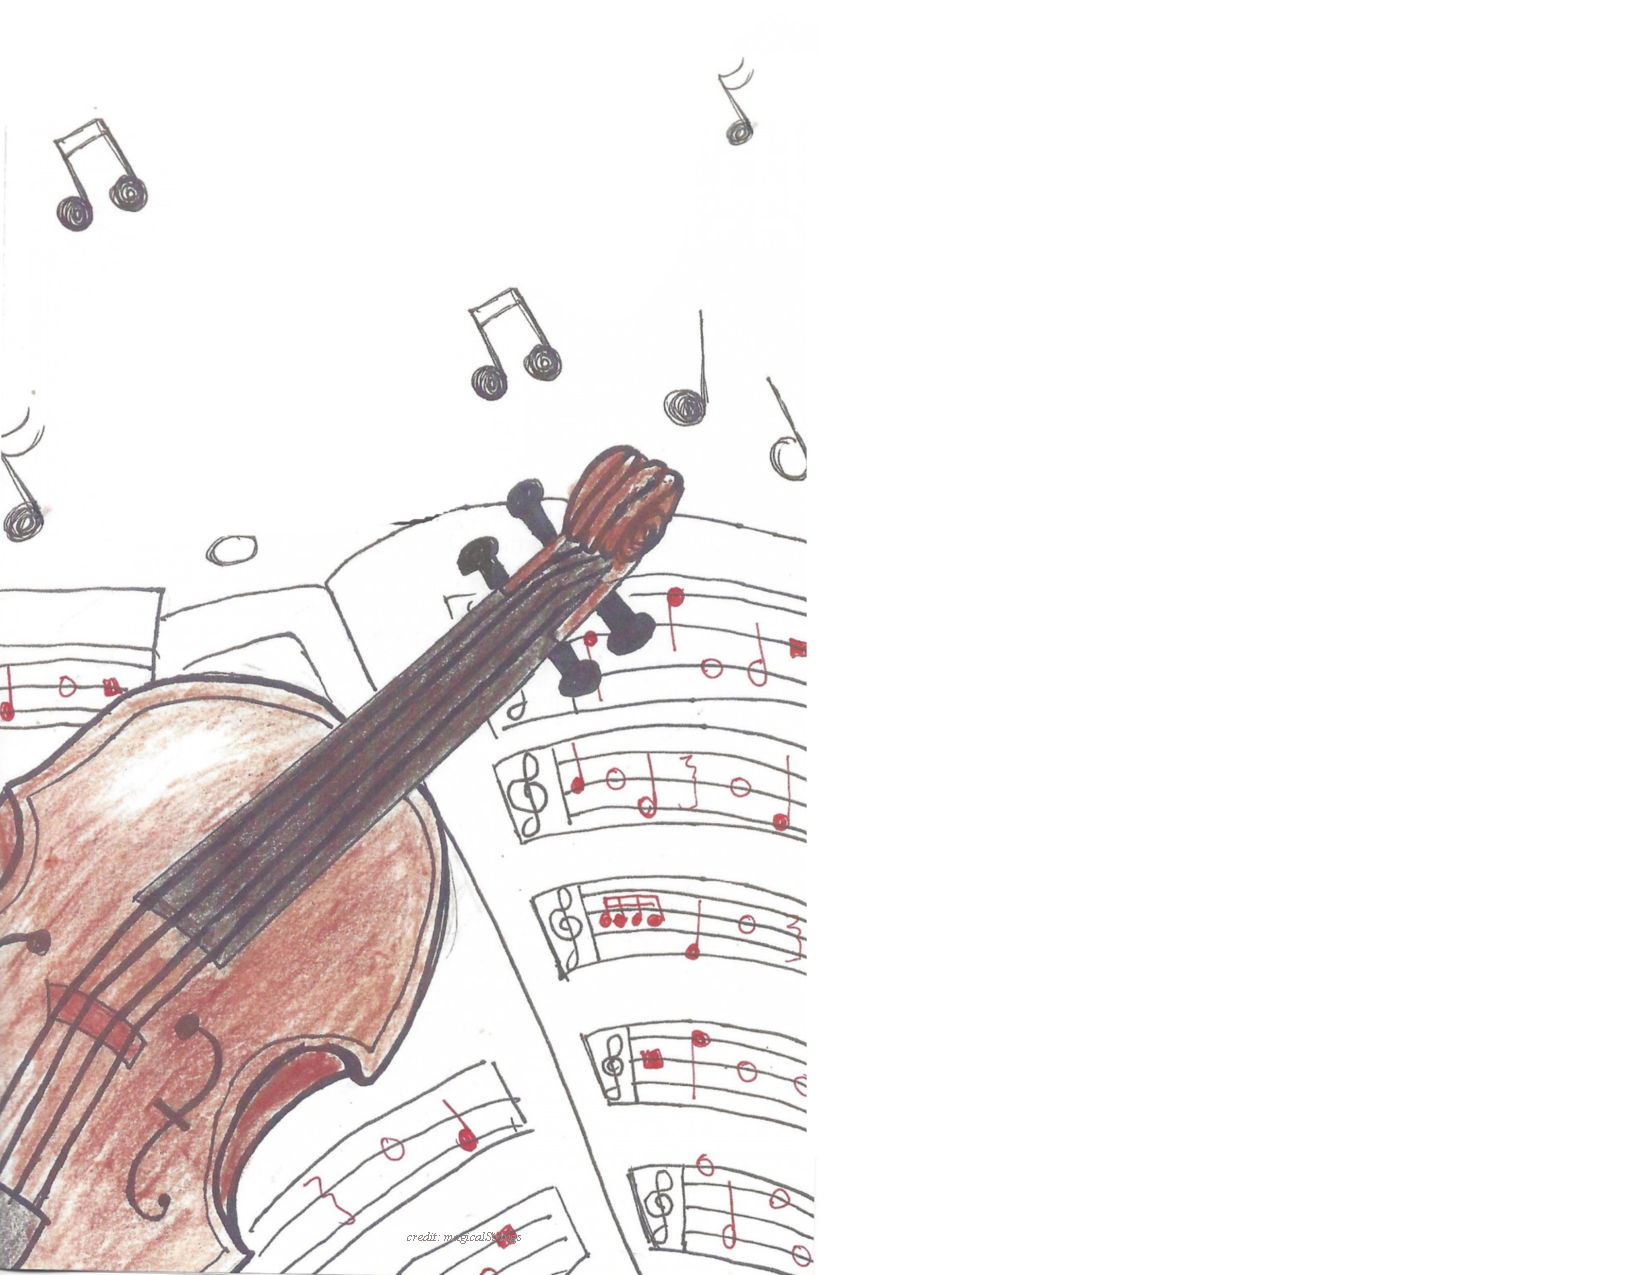
\includegraphics[height=16cm]{pg1.pdf}

\vspace{3em}

  \begin{part}[]
    \begin{composition}
    {\Large Fran\c{c}ois J. Gossec}{\normalsize{1734 -- 1829}}{\Large Gavotte}{}
    \end{composition}
\vspace{1em}    
    \begin{composition}
    {\Large Robert Schumann}{\normalsize{1810 -- 1856}}{\Large Happy Farmer}{}
    \end{composition}
\vspace{1em}     
    \begin{composition}
    {\Large Johann S. Bach}{\normalsize{1685 -- 1750}}{\Large Minuet 3}{}
    \end{composition}
\vspace{1em} 
    \begin{composition}
    {\Large Shinichi Suzuki}{\normalsize{1898 -- 1998}}{\Large Etude}{}
    \end{composition}
\vspace{1em} 
    \begin{composition}
    {\Large Shinichi Suzuki}{\normalsize{1898 -- 1998}}{\Large Andantino}{}
    \end{composition}
\vspace{1em}     
    \begin{composition}
    {\Large Shinichi Suzuki}{\normalsize{1898 -- 1998}}{\Large Perpetual Motion}{}
    \end{composition}
\vspace{1em}     
     \begin{composition}
    {\Large Shinichi Suzuki}{\normalsize{1898 -- 1998}}{\Large Allegro}{}
    \end{composition}

  \end{part}
\end{programme}

\end{document}
